%%%%%%%%%%%%%%%%%%%%%%%%%%%%%%%%%%%%%%%%%%%%%%%%
% E.Pinault-Bigeard - e.pinault-bigeard@upsti.fr
% http://s2i.pinault-bigeard.com
% CC BY-NC-SA 2.0 FR - http://creativecommons.org/licenses/by-nc-sa/2.0/fr/
%%%%%%%%%%%%%%%%%%%%%%%%%%%%%%%%%%%%%%%%%%%%%%%%
\documentclass[11pt]{article}
%%%%%%%%%%%%%%%%%%%%%%%%%%%%%%%%%%%%%%%%%%%%%%%%
% Package UPSTI_Document
%%%%%%%%%%%%%%%%%%%%%%%%%%%%%%%%%%%%%%%%%%%%%%%%

\usepackage{import}
%
%%%%%%%%%%%%%%%%%%%%%%%%%%%%%%%%%%%%%%%%%%%%%%%%
% Package UPSTI_Document
%%%%%%%%%%%%%%%%%%%%%%%%%%%%%%%%%%%%%%%%%%%%%%%%
\usepackage{subcaption}
\usepackage[usenames, svgnames, dvipsnames]{xcolor}
\usepackage{UPSTI_Document}
\usepackage{pgfplots}
\usepackage{import}
\definecolor{darkspringgreen}{rgb}{0.09, 0.45, 0.27}

\newcommandx*{\dessinRepereFigGeo}[5][1=\vx{},2=\vy{},3=\vz{},4=,5=0]
	{
		\draw [->,very thick] (0,0) -- (1,0) ;
		\draw [->,very thick] (0,0) -- (0,1) ;
    \fill[white] (0,0) circle (0.13);
    \draw [->,very thick] (0,0) circle (0.13);
    \ifnumequal{#5}{0} {% z vers nous
      \fill[black] (0,0) circle (0.03);
      \draw [->,thick] (0,0) circle (0.04);
    }{% z vers la feuille
  		\begin{scope} [rotate=45]
  			\draw [-,thick] (0,-0.12) -- (0,0.12) ;
  			\draw [-,thick] (-0.12,0) -- (0.12,0) ;
  		\end{scope}
    }
		\draw [anchor=north west] (1.1,0) node {${#1}$};
		\draw [anchor=south west] (0,1.1) node {${#2}$};
		\draw [anchor=north east] (-0.1,0) node {${#3}$};
		\draw [anchor=north west] (-0.1,-0.1) node {${#4}$};
	}

	\usepackage{array}
	\newcolumntype{L}[1]{>{\raggedright\let\newline\\\arraybackslash\hspace{0pt}}m{#1}}
	\newcolumntype{C}[1]{>{\centering\let\newline\\\arraybackslash\hspace{0pt}}m{#1}}
	\newcolumntype{R}[1]{>{\raggedleft\let\newline\\\arraybackslash\hspace{0pt}}m{#1}}

	\usepackage{pifont}% http://ctan.org/pkg/pifont
\newcommand{\cmark}{\color{green}\ding{51}}%
\newcommand{\xmark}{\color{red}\ding{55}}%
\newcommand{\fmark}{\ding{229}}%
\newcommand{\itemc}{\item[\cmark]}%
\newcommand{\itemx}{\item[\xmark]}%
\newcommand{\itemf}{\item[\fmark]}%

\usepackage{tikz-timing}
\usepackage{circuitikz}
\usepackage{pdfpages}
%---------------------------------%
% Paramètres du package
%---------------------------------%

% Version du document (pour la compilation)
% 1: Document prof
% 2: Document élève
% 3: Document à publier
\newcommand{\UPSTIidVersionDocument}{2}

% Classe
% 1: PTSI				6: PSI*			11: TSI2		16: Spé
% 2: PT	(par défaut)	7: MPSI			12: ATS
% 3: PT*				8: MP			13: PC
% 4: PCSI				9: MP*			14: PC*
% 5: PSI				10: TSI1		15: Sup
%\newcommand{\UPSTIidClasse}{2}



% Matière
% 1: S2I (par défaut)    2: IPT     3: TIPE
% 6: Vie au lycée
\newcommand{\UPSTIvariante}{5}
\newcommand{\UPSTIidMatiere}{0}
\newcommand{\UPSTIintituleMatiere}{Automatique}
\newcommand{\UPSTIsigleMatiere}{Autom}
% Type de document
% 0: Custom*				7: Fiche Métho de			14: Document Réponses
% 1: Cours (par défaut)		8: Fiche Synthèse    		15: Programme de colle
% 2: TD     				9: Formulaire
% 3: TP						10: Memo
% 4: Colle					11: Dossier Technique
% 5: DS						12: Dossier Ressource
% 6: DM						13: Concours Blanc
% * Si on met la valeur 0, il faut décommenter la ligne suivante:
%\newcommand{\UPSTItypeDocument}{Custom}
\newcommand{\UPSTIidTypeDocument}{1}

% Titre dans l'en-tête


% Titre dans l'en-tête

\newcommand{\UPSTIvariante}{5}

\newcommand{\UPSTItitreEnTete}{Automatisme industriel}
%\newcommand{\UPSTItitreEnTetePages}{}
\newcommand{\UPSTIsousTitreEnTete}{Introduction aux API}


% Titre
%\newcommand{\UPSTItitrePreambule}{Automatisme industriel}
\newcommand{\UPSTItitre}{La programmation d'un Automate Industriel}

% Durée de l'activité (pour DS, DM et TP)
\newcommand{\UPSTIduree}{3h30}

% Note de bas de première page
%\newcommand{\UPSTInoteBasDePremierePage}{Geoffrey Vaquette}
% Numéro (ajoute " n°1" après DS ou DM)
\newcommand{\UPSTInumero}{2}

% Numéro chapitre
%\newcommand{\UPSTInumeroChapitre}{1}

% En-tête customisé
%\newcommand{\UPSTIenTetePrincipalCustom}{UPSTIenTetePrincipalCustom}

% Message sous le titre
%\newcommand{\UPSTImessage}{Message sous le titre}


% Référence au programme
%\newcommand{\UPSTIprogramme}{\EPBComp \EPBCompP{B1-02}, \EPBCompP{B2-49}, \EPBCompS{B2-50}, \EPBCompS{B2-51}, \EPBCompP{C1-07}, \EPBCompP{C1-08}}

% Si l'auteur n'est pas l'auteur par défaut
%\renewcommand{\UPSTIauteur}{WWOOOOOOWW}

% Si le document est réalisé au nom de l'équipe
%\newcommand{\UPSTIdocumentCollegial}{1}

% Source
\newcommand{\UPSTIsource}{G. Vaquette}

% Version du document
\newcommand{\UPSTInumeroVersion}{1.0}

%-----------------------------------------------
\UPSTIcompileVars		% "Compile" les variables
%%%%%%%%%%%%%%%%%%%%%%%%%%%%%%%%%%%%%%%%%%%%%%%%


% Titre
%\newcommand{\UPSTItitrePreambule}{Automatisme industriel}
\newcommand{\UPSTItitre}{Exercice de synthèse} 
\usetikzlibrary{arrows,automata,circuits.plc.ladder}

\newlength{\ladderskip}
\setlength{\ladderskip}{5\tikzcircuitssizeunit} % 5\tikzcircuitssizeunit = 35pt
\newlength{\ladderrungsep}
\setlength{\ladderrungsep}{.2\ladderskip}
\def\ladderrungend#1{\pgftransformyshift{-#1\ladderskip-\ladderrungsep}}

\ctikzset{
	logic ports=ieee,
	logic ports/scale=0.7,
}



\newcommand{\automaintienMachineEtat}[0]{
\begin{tikzpicture}[->,>=stealth',shorten >=1pt,auto,node distance=3cm,
                    semithick]
  %\tikzstyle{every state}=[fill=none,draw=none,text=white]

  \node[initial,state] (A)              {M1};
  \node[state]         (B) [right of=A] {M2};

  \path (A) edge [bend left]  node {$B_pM$} (B)
        (B) edge [bend left]  node {$B_pA$} (A);
\end{tikzpicture}
}


%%%%%%%%%%%%%%%%%%%%%%%%%%%%%%%%%%%%%%%%%%%%%%%%
% Début du document
%%%%%%%%%%%%%%%%%%%%%%%%%%%%%%%%%%%%%%%%%%%%%%%%
\begin{document}
\UPSTIbuildPage

%\UPSTIobjectif{Durant cette activité, nous allons analyser une trame pour l'envoi d'informations sur une étiquette.}

\tableofcontents
%\pagebreak

\pagebreak
\section{Introduction}
Cette séance de synthèse avant la semaine de TP test a pour objectif de revoir et d'appliquer les notions vues jusqu'ici. Elle portera sur un portail automatique.

\begin{figure}[ht]
	\centering
	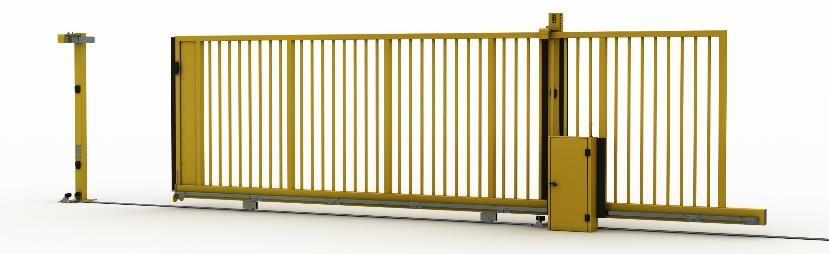
\includegraphics[width=.85\linewidth]{images/portail.jpg}
	\caption{Partie opérative du portail automatique}
	\label{fig:schemaPartieOperative}
\end{figure}

Le système consiste en un portail automatisé composé d'une barrière coulissante. Cette barrière est actionnée par un moteur à courant continu. Deux capteurs fin de course sont positionnés en bout du portail afin de détecter l'ouverture et la fermeture complète du portail.

L'utilisateur commande le portail à l'aide de deux boutons poussoir : \textit{BPO} pour l'ouverture et \textit{BPF} pour la fermeture.

Pour des questions de sécurité, un voyant lumineux clignote lorsque le portail est en mouvement et une barrière infrarouge détecte le passage d'une personne devant le portail lors de sa fermeture.

\section{Travail en classe}
\begin{UPSTIactivite}
	\UPSTIquestion{Faire la liste des capteurs du système}

	\UPSTIquestion{En déduire le nombre d'entrées logiques, numériques et analogiques}

	\UPSTIquestion{Faire la liste des actionneurs du système}

	Afin de commander le moteur dans les deux sens de rotation, on se propose d'utiliser deux relais. Ces deux relais possèdent des contacts normalement fermé et normalement ouvert.

	\UPSTIquestion{En déduire le nombre de sorties logiques, numériques et analogiques}

	\UPSTIquestion{Faudra-t-il installer des modules complémentaires sur le LOGO pour commander le portail ?}

\end{UPSTIactivite}



\begin{UPSTIactivite}
	\UPSTIquestion{Dessiner le cablâge des capteurs sur les entrées de l'automate LOGO}
	\UPSTIquestion{Dessiner le cablâge des sorties (lumière et relais)}
	\UPSTIquestion{Dessiner le schéma des contacts pour les moteurs}
\end{UPSTIactivite}

\UPSTIboiteCentrale{Cahier des charges}{
	\begin{itemize}
		\item A l'appui sur le bouton poussoir d'ouverture, le portail s'ouvre complètement
		\item Ensuite, à l'appui sur le bouton poussoir de fermeture, le portail se ferme complètement
		\item Lorsque le portail est en mouvement, la lumière clignote
	\end{itemize}
}
\begin{UPSTIactivite}
	\UPSTIquestion{Dessiner une machine à état codant le comportement précédent.}
\end{UPSTIactivite}

\section{Travaux pratiques}
\subsection{Cahier des charges principal}
\begin{UPSTIactivite}
	\UPSTIquestion{Réaliser le cablâge de l'activité précédente et faire vérifier par l'enseignant}
	\UPSTIquestion{Implémenter la machine à état correspondante}
\end{UPSTIactivite}

\UPSTIboiteGenerique{Conseil pour les machine à état}{\bcplume}{
	Lors de l'implémentation des machines à état, respecter la structure donnée en cours et ajouter des commentaires sur les Mementos correspondant aux états rendra la tâche plus simple et augmentera sa lisibilité. 
}

\subsection{Fermeture automatique}
\UPSTIboiteCentrale{Cahier des charges - suite}{
	\begin{itemize}
		\item Une fois ouvert, le portail se ferme aussi automatiquement après 5 secondes
		\item Durant la fermeture du portail, si une personne passe sur le trajet de la barrière, il se ré-ouvre 
	\end{itemize}
}


\begin{UPSTIactivite}
	\begin{itemize}
		\item Modifier la machine à état pour respecter le cahier des charges ci-dessus
		\item Implémenter ce cahier des charges
	\end{itemize}

	Afin d'effectuer de précieuses économies, on prend la décision de retirer un des deux capteurs fin de courses. Un seul capteur fin de course sert à la fois pour la position ouverte et pour la position fermée. 

	\begin{itemize}
		\item Effectuer le changement et débrancher le capteur non utilisé.
	\end{itemize}
\end{UPSTIactivite}
\subsection{Mode \textit{rester ouvert}}
\UPSTIboiteCentrale{Cahier des charges - suite}{
	\begin{itemize}
		\item Une fois ouvert, si on appui à nouveau sur le bouton d'ouverture, le portail entre dans un mode où il attend un appui sur le bouton de fermeture pour se fermer
	\end{itemize}
}


\begin{UPSTIactivite}
	\begin{itemize}
		\item Modifier la machine à état pour respecter le cahier des charges ci-dessus
		\item Implémenter ce cahier des charges
	\end{itemize}
\end{UPSTIactivite}
\end{document}
